\section{Related Works}%
\label{sec:related_works}
%
\begin{figure}[t]
    \centering
    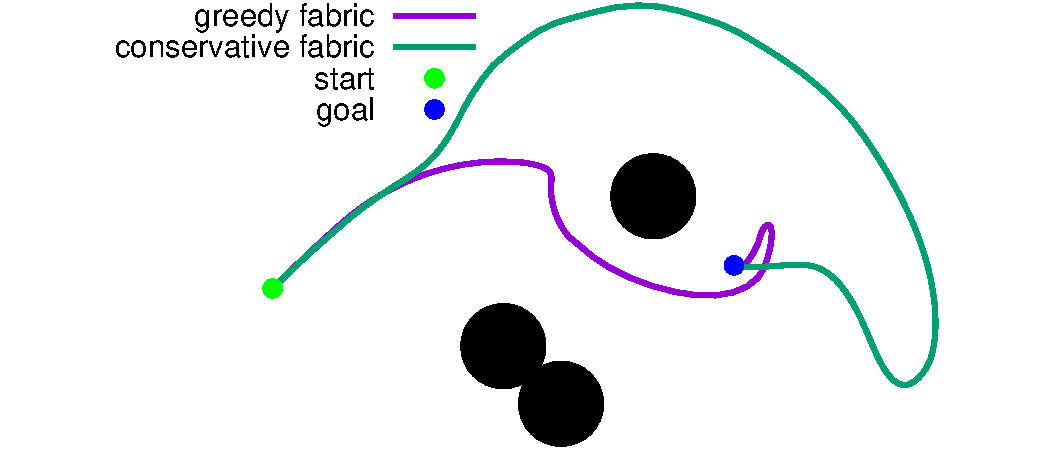
\includegraphics[width=0.8\linewidth]{effect_tuning}
    \captionsetup{belowskip=-10pt}
    \caption{Two different parameter sets for optimization fabrics given the same problem. While the greedy tuning
    is more aggressive (purple), the more conservative tuning results in a smoother trajectory (green).}
    \label{fig:effect_tuning}
\end{figure}
%

\subsection{Autotuning for trajectory generation}
%
Autotuning can be beneficial for trajectory generation when using model predictive control.
In \cite{loquercio_autotune_2022}, an autotuned
model predictive controller has outperformed a manual tuned controller of the same kind by 
25\%. Jointly optimizing parameters and the model of the controller, \textit{AutoMPC} 
showed the benefit of parameter tuning in the context of simultaneous system
identification and control \cite{edwards_automatic_2021}. These methods are explicitly 
formulated for model predictive control and do not transfer easily to other trajectory generation
methods. In contrast, we propose a generic parameter optimization approach to trajectory generation.

\subsection{Hyperparameter tuning in machine learning}
%
Within the machine-learning field, hyperparameter tuning has shown to be highly 
important for all different kinds of applications \cite{yang2020hyperparameter,hutter_automated_2019,optuna}. 
Parameter optimization aims to minimize 
training costs while achieving the best possible performance. Hyperparameter tuning 
is most valuable in extremely
costly applications such as reinforcement learning \cite{zoph_neural_2017}. Generally, two different search
algorithms have been investigated: grid search and random search \cite{bergstra_random_nodate}.
Current state-of-the-art methods for parameter search are based on 
random search with a Bayesian optimizer \cite{optuna,bergstra_algorithms_nodate}.
While the machine-learning community has largely agreed on the importance of
parameter tuning, systematic tuning of trajectory generation methods are not well established. 
In this paper, we showcase, with the example of optimization fabrics, how important 
parameter tuning is and how trajectory generation can benefit from it.
